\documentclass[10pt,a4paper]{article}

\usepackage[utf8]{inputenc}
\usepackage[T1]{fontenc}
\usepackage[french]{babel}
\usepackage[margin=0.9cm]{geometry} % Marges fines pour tenir sur une page
\usepackage{titlesec}
\usepackage{enumitem}
\usepackage{hyperref}
\usepackage{xcolor}
\usepackage{fontawesome5} % Pour les icônes
\usepackage{graphicx} % Pour inclure des images

% Police Serif (standard LaTeX, très académique)
\usepackage{lmodern}

% Couleurs
\definecolor{primary}{RGB}{35, 75, 145} % Un bleu classique et élégant
\definecolor{darkgray}{RGB}{51, 51, 51}

\hypersetup{
    colorlinks=true,
    linkcolor=primary,
    filecolor=primary,
    urlcolor=primary,
}

% Format des titres de sections (Petites Capitales + ligne)
\titleformat{\section}{\large\scshape\color{primary}}{}{0em}{}[\titlerule]
\titlespacing{\section}{0pt}{6pt}{3pt}

% Espacement des listes
\setlist[itemize]{leftmargin=1.5em, itemsep=0pt, topsep=1pt, parsep=0pt, partopsep=0pt}

% Séparateur personnalisé
\newcommand{\separator}{ \ | \ }

\begin{document}
\pagestyle{empty} % Retire les numéros de page

% ==========================================
% EN-TÊTE
% ==========================================
\noindent
\begin{minipage}[t]{0.75\textwidth}
{\Huge \textbf{\textcolor{primary}{Noah CIVILISE}}}\\[2pt]
{\footnotesize
\faPhone \ +33 6 60 39 97 86 \separator
\faMapMarker \ Bordeaux / Paris \separator
\faEnvelope \ \href{mailto:civilise.noah@gmail.com}{civilise.noah@gmail.com} \separator
\faLinkedin \ \href{https://www.linkedin.com/in/noah-civilise/}{noah-civilise} \separator
\faGithub \ \href{https://github.com/Noah30c}{Noah30c}
}\\[2pt]
{\large Étudiant en 5\textsuperscript{ème} année à EPITA -- Ingénierie Informatique}
\end{minipage}%
\begin{minipage}[t]{0.25\textwidth}
\vspace{-0.7cm}
\raggedleft
% L'option trim prend 4 valeurs : gauche, bas, droite, haut.
% Ajuste ces valeurs (en cm ou pt) pour rogner selon ton besoin.
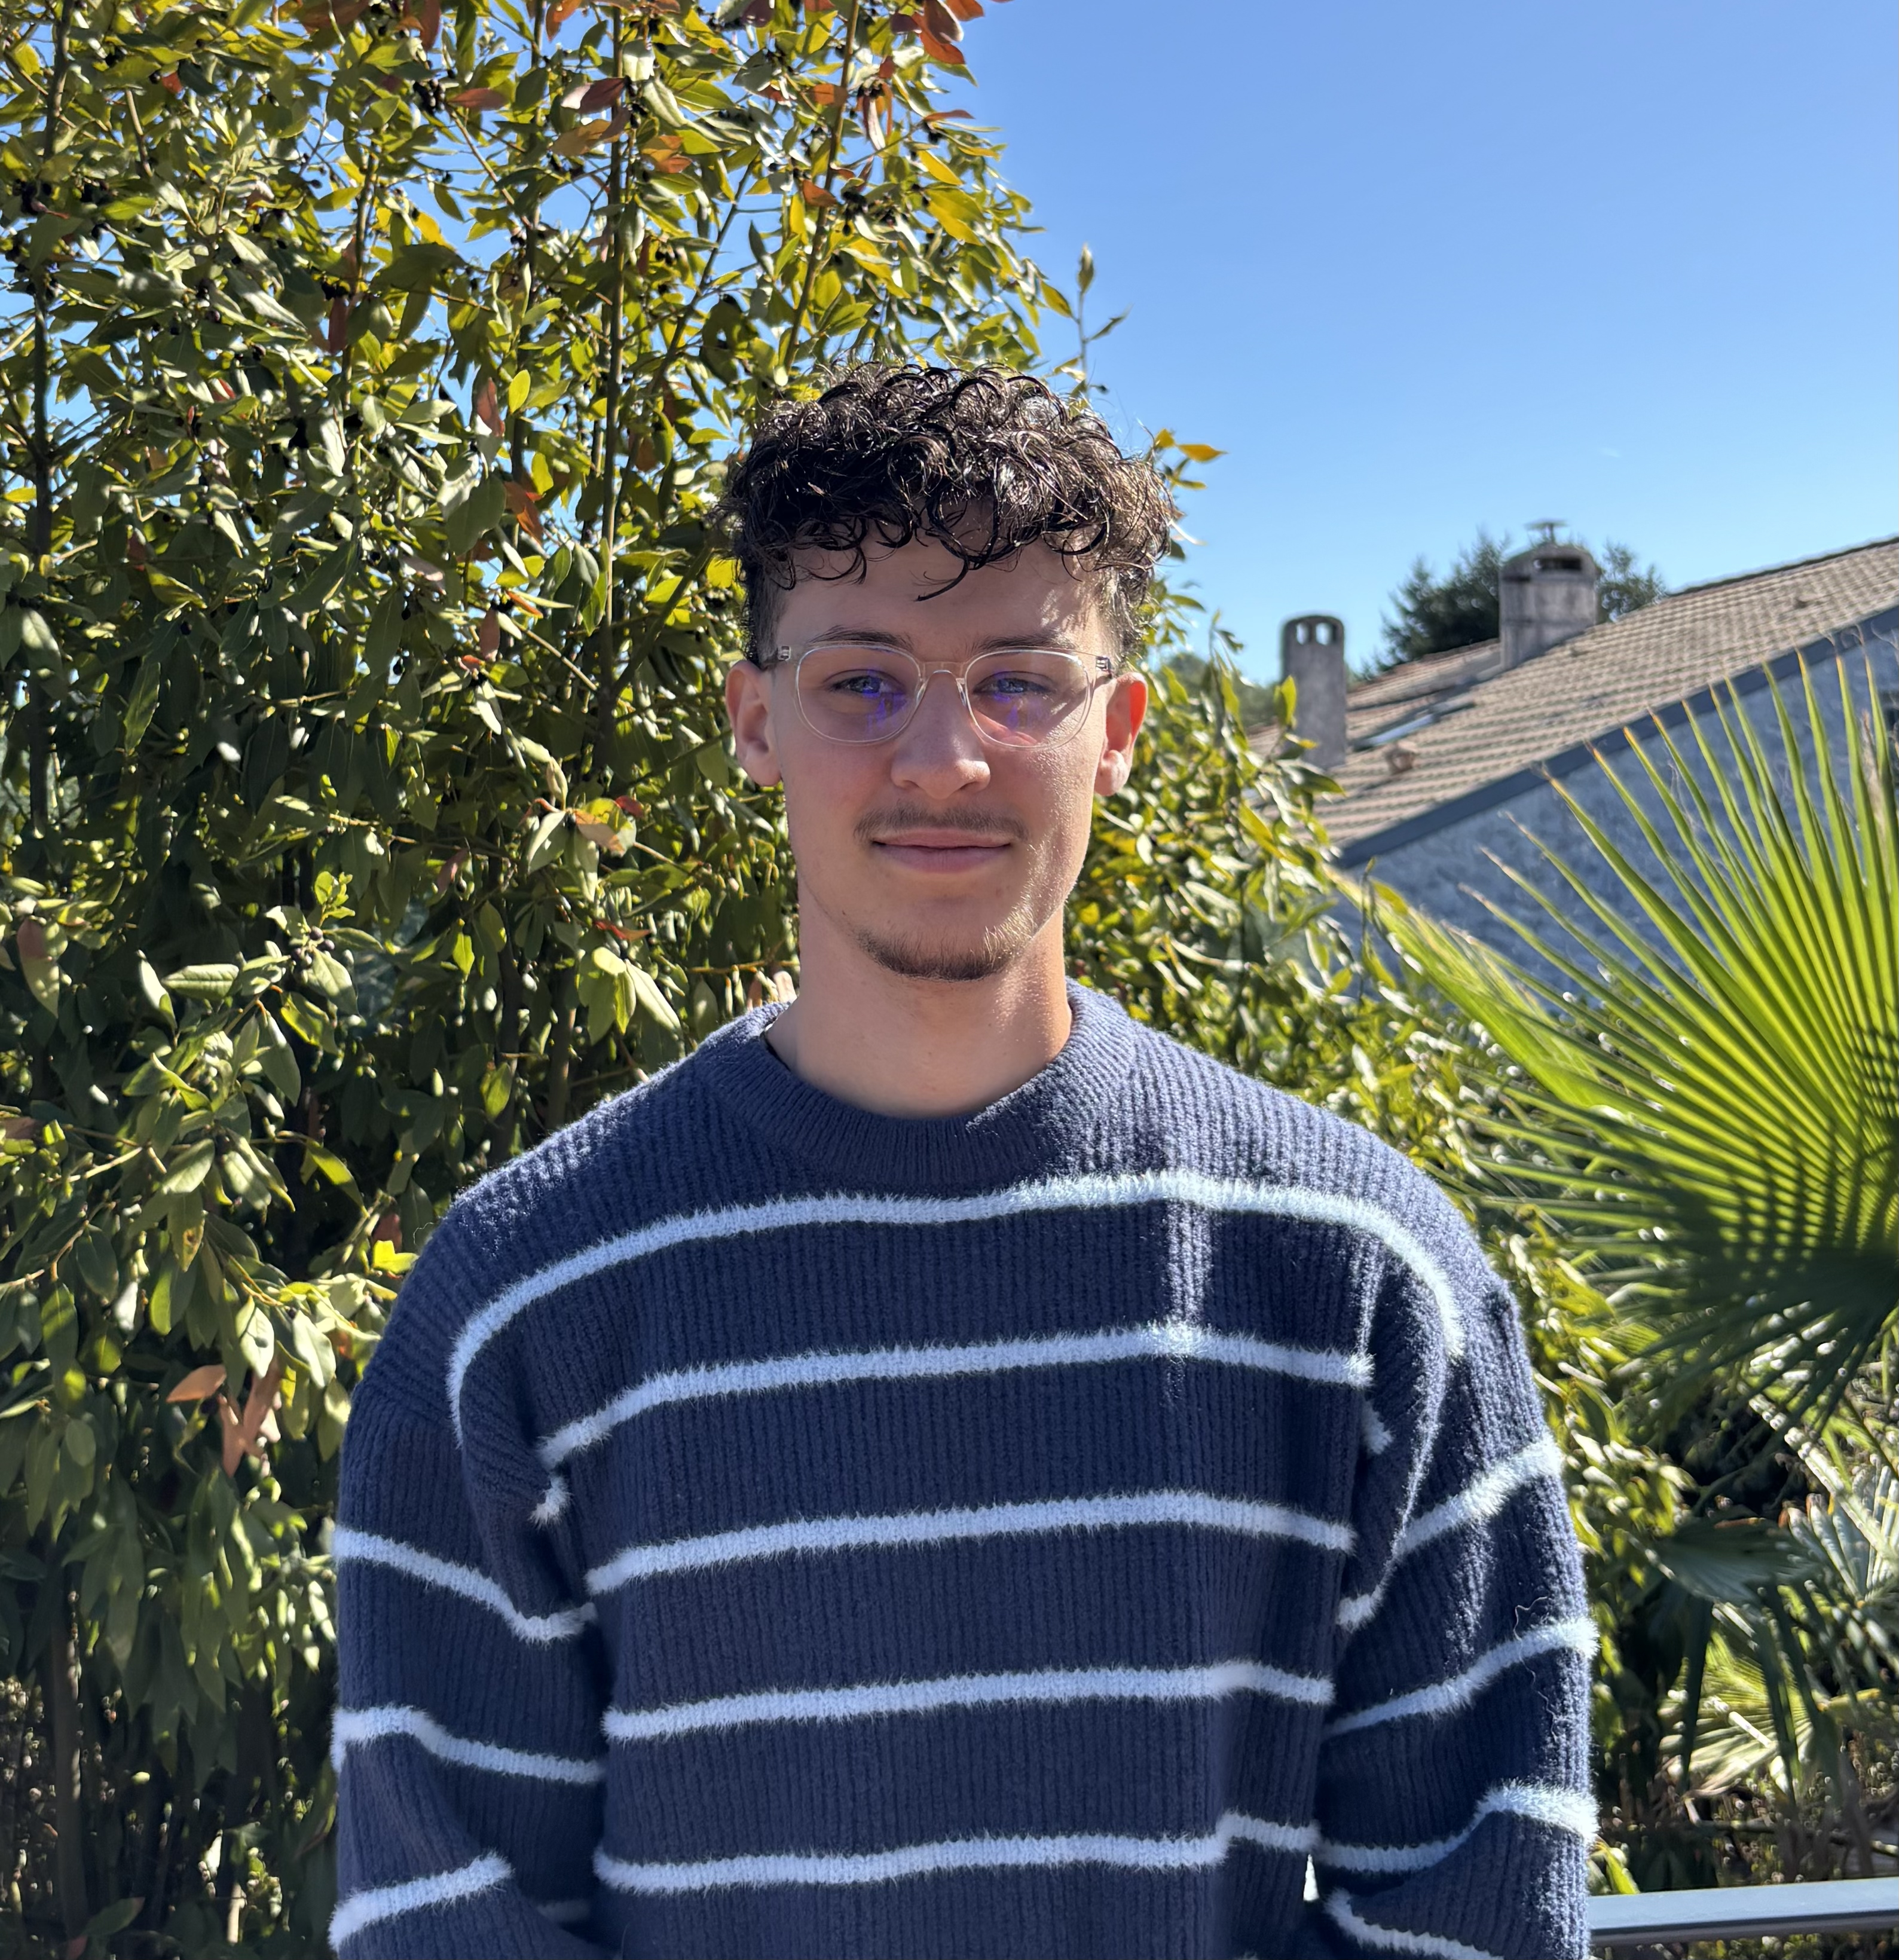
\includegraphics[trim=4.5cm 6cm 4.5cm 4cm, clip, width=2.7cm]{../images/moi-3.jpg}
\end{minipage}

\vspace{0.1cm}

% ==========================================
% OBJECTIF
% ==========================================
\section*{Objectif}
\noindent
Je recherche un stage de fin d'études de 6 mois en Intelligence Artificielle ou en Traitement d'Image à partir de février 2027 sur Bordeaux ou Paris. Curieux, adaptable et motivé, je souhaite approfondir mes compétences dans ces domaines au sein d'un environnement stimulant.

% ==========================================
% EXPÉRIENCES PROFESSIONNELLES
% ==========================================
\section*{Expériences Professionnelles}

\noindent
\textbf{Projet de Fin d'Études (PFEE) -- Ingénieur Réalité Virtuelle} \hfill \textit{Fev 2026 - Aujourd'hui} \\
\textit{\textbf{Dassault Systèmes}} \\
\textit{Conception d'un outil d'aide à la navigation (Minimap) en Réalité Virtuelle (WebXR) pour environnements 3D complexes.}
\begin{itemize}
    \item Développement WebXR (Three.js, TypeScript) d'une Minimap dynamique en réalité virtuelle.
    \item Implémentation d'algorithmes 3D ("World Detection") et optimisation asynchrone via WebWorkers.
\end{itemize}

\vspace{0.15cm}

\noindent
\textbf{Data Science \& Generative AI Intern} \hfill \textit{Sept 2025 -- Janv 2026} \\
\textit{\textbf{Compagnie Européenne de Garanties et Cautions (Groupe BPCE)}}
\begin{itemize}
    \item \textbf{Architecture RAG \& LLM} : Conception "from scratch" d'un pipeline d'extraction d'informations sur des centaines de bilans PDF (SentenceTransformer, Qdrant, LLM).
    \item \textbf{Fiabilisation \& MLOps} : Validation stricte des données générées (JSON, Pydantic, Luhn) et suivi des métriques de confiance (77.1\%) sur interface Streamlit.
    \item \textbf{Automatisation \& NLP} : Développement d'un outil de contrôle croisant données Excel et textes de PDF analysés par LLM (Gain de temps : >60\%).
    \item \textbf{Industrialisation} : Déploiement d'exécutables autonomes (PyInstaller) pour s'affranchir des contraintes IT métier, et orchestration sur Dataiku.
    \item \textbf{Business Intelligence} : Modélisation en étoile et tableau de bord Power BI (DAX) automatisant la détection des dérives des règles d'octroi de cautionnement.
\end{itemize}

\vspace{0.15cm}

\noindent
\textbf{Tuteur} \hfill \textit{2022 -- 2025} \\
\textit{BackToBasics, EPITA}
\begin{itemize}
    \item Tutorat en algorithmique, programmation et mathématiques (séances individuelles et en groupe).
\end{itemize}

% ==========================================
% PROJETS TECHNIQUES
% ==========================================
\section*{Projets Techniques}

\noindent
\textbf{Automatic License Plate Recognition (ALPR)} \hfill \textit{C++, Python, OpenCV, ML} \\
Développement "from scratch" d'une pipeline de localisation de plaques d'immatriculation sans Deep Learning. Prototypage (Python) puis portage bas niveau (C++) pour l'optimisation (librairie MyCV, Random Forest, CI/CD). Traitement < 380ms avec 93\% d'exactitude.


\noindent
\textbf{DermScan (IA Médicale)} \hfill \textit{Python, OpenCV, FastAPI, RabbitMQ, Docker} \\
Application distribuée d'aide au diagnostic dermatologique (règle ABCDE). Pipeline de vision par ordinateur (K-Means, PCA) et Machine Learning (MLP, sensibilité >85\%) orienté explicabilité. Architecture microservices asynchrones avec CI/CD complète.


\noindent
\textbf{Filtre GStreamer (CUDA)} \hfill \textit{C++, CUDA, GStreamer} \\
Optimisation GPGPU d'un filtre vidéo de détection de mouvement. Pipeline de traitement temps réel avec accélération CUDA (CUDA Graphs, mémoire Pinned).


\noindent
\textbf{Compilateur Tiger} \hfill \textit{C++, Flex/Bison, LLVM} \\
Développement en équipe d'un compilateur complet pour le langage objet Tiger. Architecture modulaire : analyse lexico-syntaxique, vérification sémantique et génération de code (LLVM IR). Implémentation d'optimisations (inlining, analyse d'échappement).

% ==========================================
% FORMATION
% ==========================================
\section*{Formation}

\noindent
\textbf{EPITA – École d'ingénieurs en informatique} \hfill \textit{2022 -- 2027} \\
Traitement \& synthèse d’images, vision par ordinateur, deep learning, IA, calcul GPU - \textbf{GPA : 4.0} \hfill \textit{Le Kremlin-Bicêtre}



\noindent
\textbf{Universidad del País Vasco} \hfill \textit{2024} \\
Échange académique \hfill \textit{San Sebastián, Espagne}



\noindent
\textbf{Baccalauréat Scientifique} \hfill \textit{2019 -- 2022} \\
Maths et NSI -- \textbf{Mention Très Bien} \hfill \textit{Montigny-Le-Bretonneux}

% ==========================================
% COMPÉTENCES
% ==========================================
\section*{Compétences}
\noindent
\textbf{Vision par ordinateur \& IA : }  Traitement d’images, Deep learning, PyTorch, YOLO, RAG, NLP, ML \\
\textbf{Programmation:} Cuda, GStreamer, OpenGL, GLSL, C++, C, C\#, Python, JS, Java, Bash, HTML/CSS \\
\textbf{Outils \& Frameworks :} OpenCV, React, FastAPI, Docker, RabbitMQ, CMake, Git, CI/CD \\
\textbf{Soft skills :} Adaptabilité, Travail d'équipe, Autonomie, Résolution de problèmes \\
\textbf{Langues :} Français (Natif), Anglais (TOEIC 900/990 - Courant), Espagnol (B1)
\end{document}